\chapter{Introdução}

\section{Enquadramento\label{se:enquadramento}}
Esta dissertação enquadra-se no âmbito do projeto \href{https://traderes.eu/}{TradeRES}, que visa o estudo de um sistema de mercado eléctrico capaz de atender às necessidades da sociedade num sistema quase totalmente renovável, tendo as características para se integrar nos \href{https://ods.pt/ods/}{ \gls{ODS}} \ref{fig:ODS}.\par
O estudo da acessibilidade das energias renováveis ao mercado vigente integra-se nos \gls{ODS} n$^{\circ}$7, “Energia Renováveis e Acessíveis”, indo directamente de encontro a um dos pontos deste objectivo: 7.2.1 “Peso das energias renováveis no consumo total final de energia”. Por meio deste objectivo, a participação das renováveis no mercado faz também cumprir, embora indiretamente, o objectivo n$^{\circ}$8 “Trabalho Digno e Crescimento Económico”, através do ponto 8.4, onde, neste último, é dada primazia à eficiência dos recursos globais no consumo e na produção. Esta contribuição indireta ocorre através da diminuição do uso de energias não limpas, justificadas por um maior uso das renováveis, melhorando a gestão de recursos, e baixando o consumo de recursos naturais não renováveis.\par
Por último, no âmbito do presente estudo, podemos igualmente incluir o objectivo n$^{\circ}$13, “Acção Climática”, no qual, referimos, não só a diminuição de consumo de recursos finitos, mas ainda, a melhor gestão de recursos renováveis, promovendo o planeamento e estratégias de combate a emissões de gases de efeito estufa.\par

\begin{figure}[h]
    \centering
    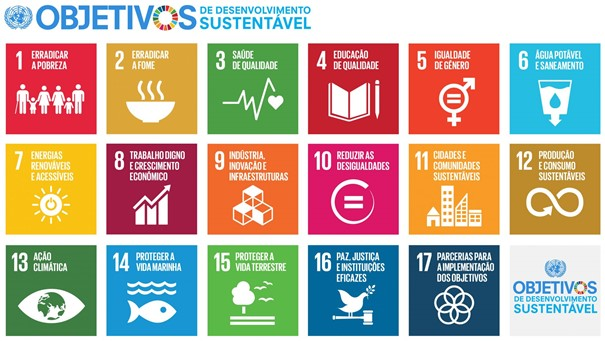
\includegraphics{Imagens/DesenvolvimentoSustentavel.jpg}
    \caption{Objectivos de Desenvolvimento Sustentável da ONU}
    \label{fig:ODS}
\end{figure}

\section{Objetivos e Perguntas de Pesquisa\label{se:objetivos}}

Foram aprovadas a nível europeu (2020)\cite{52020DC0299} sugestões de alterações aos serviços de sistema, que serão seguidas pelos Estados-Membros. Nesta dissertação, será realizada a aplicação dessas sugestões, identificando as melhorias em relação ao \textit{design} actual e avaliando se as novas sugestões serão suficientes para garantir a operação de um sistema elétrico \textasciitilde100\% renovável, potencialmente identificando ações adicionais para garantir a robustez e segurança do sistema elétrico sem o uso de combustíveis fósseis.\par
A penetração das \gls{vRES} no sistema de energia eléctrica trouxe maior incerteza na previsão em mercados de energia, pois estas estão mais sujeitos a elementos não controláveis como a velocidade do vento ou a radiação solar incidente.\par
As seguintes perguntas servirão de guia nesta pesquisa:\par

\begin{enumerate}[label=\alph*)]
  \item Podemos reduzir a incerteza na produção criada pela participação das \gls{vRES} nos sistemas de energia? 
  \item A alocação dinâmica pode ter um efeito positivo no mercado de reservas?
  \item É possível prever a necessidade de reserva necessária baixando a alocação desperdiçada?
\end{enumerate}

Para responder às perguntas \textit{supra} referidas, utilizaremos dados de previsão de geração de energia renovável para estimar a energia necessária para alocação secundária. Actualmente, os valores de previsão desse mercado estão distantes do consumo real, o que resulta em alocações no dia anterior que não estão em conformidade com as necessidades reais.\par
O objetivo deste trabalho é criar métodos de previsão para o dia seguinte, da necessidade de alocação de banda de reserva secundária, de modo a alocar banda suficiente e, simultaneamente, baixar a alocação em excesso, usando dados históricos das mesmas.\par
Iremos explorar a optimização da fórmula de alocação de banda de reserva da REN, testando novos valores para o parâmetro horário da mesma.\par
Utilizando técnicas de \textit{machine learning} vamos criar um modelo para a previsão de alocação necessária do dia seguinte.\par
Previsões mais exactas tornam possível uma melhor gestão das alocações, resultando num menor gasto de recursos energéticos e financeiros.\par

\section{Organização do Documento \label{se:organização}}

Este documento está dividido em capítulos. Sendo que os primeiros apresentam uma introdução às ideias e temas no 1, o estado de arte dos temas na literatura publicada, seguido de uma contextualização do tema do trabalho proposto no capítulo 2. Dentro da contextualização é de forma geral apresentado os mercados de energia, os sistemas de reserva, e os métodos de previsão para os mesmos, dentro destes o uso de fórmulas e o uso de \textit{machine learning}, formulando aqui a motivação e caminho de estudo.\par
No capítulo 3 apresentamos no sub-capítulo Ferramentas as bibliotecas criadas em \textit{python} para o presente estudo.
Segue o sub-capítulo Métodos onde abordamos os diferentes estudos presentes, como serão dirigidos e condições a alcançar. Dividindo o trabalho em estudos distintos para o tipo de previsões apresentadas no capítulo 2.
Métricas e Dados intitula o capítulo 4 que começa numa dissecção das métricas aplicadas ao longo das experiências e como estas influenciam a mesma, terminando num estudo geral dos dados utilizados, seus tratamentos e elações iniciais de análise. Apresentado também o que é usado como treino e como validação para as experiências.
No capítulo 5 são apresentados os resultados da experiência completa, incluindo as métricas apresentadas, apresentado gráficos de séries temporais das previsões conseguidas. Dando realce aos melhores modelos e optimizações conseguidos.
Termina com um breve capítulo conclusivo dando um pouco mais de contexto aos resultados, apresentando possíveis caminhos futuros de melhoria dos mesmos e discutindo o impacto de \textit{machine learning} no futuro das energias renováveis e consequentemente nos mercados de reserva.

% Os dois capítulos seguintes apresentam os dois diferentes estudos. No \hyperref[ch:estudo_1]{capítulo 4} é definido e apresentado o resultado do estudo da estimativa do parâmetro $\rho$ da fórmula de estimativa da \gls{REN}.\par
% No \hyperref[ch:estudo_2]{capítulo 5} explora-se o segundo estudo, o dimensionamento dinâmico da alocação necessária. São apresentados os dados utilizados com um estudo preliminar sobre os mesmos, e o tratamento necessário para usar nos modelos.\par
% No \hyperref[ch:ferramentas]{capítulo 6} as ferramentas de programação criadas para realizar a mesma.\par
% Os 3 capítulos seguintes são os descritivos da experiência em si. \hyperref[ch:metricas]{Capítulo 7} são as métricas usadas e criadas para a validação da experiência, \hyperref[ch:metodos]{capítulo 8} é a estrutura e parametrização da mesma, e \hyperref[ch:resultados_discussao]{capítulo 9} apresenta os resultados.\par
% Termina com um \hyperref[ch:conclusao]{capítulo conclusivo} onde são avaliadas as experiências como um todo, e o seu impacto no âmbito dos mercados de reserva.\par